\documentclass[final]{beamer}

% Set the dimensions of the poster
\usepackage[orientation=landscape,size=a2,scale=1.5,debug]{beamerposter}  % e.g. custom size poster
\title[R\&P peace]{New evidence of violent conflicts between Rabbitskinners and Poppychewers}

\author[Pants]{Fancy Pants \& Parlanchín Gutiérrez Pascual Torres}
\date{April 2023}

\definecolor{redcaa}{RGB}{152,0,34}

% Set the font sizes for the headings and text
\setbeamerfont{title}{size=\huge}
\setbeamerfont{author}{size=\large}
\setbeamerfont{institute}{size=\large}
%\setbeamerfont{block title}{size=\Large}
%\setbeamerfont{block body}{size=\large}


% Remove the navigation symbols at the bottom of the poster
\setbeamertemplate{navigation symbols}{}

% Set the background color of the poster
\setbeamercolor{background canvas}{bg=redcaa}
\setbeamercolor{block,sep=2pt}{bg=white}
\setbeamercolor{structure}{bg=redcaa}

\setbeamercolor{block}{fg=black}
\setbeamercolor{title}{bg=white}
\setbeamercolor{block title}{fg=redcaa,bg=white}
\setbeamercolor{block body}{use=block title,bg=block title.bg}
\setbeamercolor{separation line}{fg=redcaa,bg=redcaa}
\setbeamercolor{block separation line}{fg=redcaa,bg=redcaa}
\setbeamercolor{footline}{fg=redcaa,bg=white}
\setbeamercolor{footlinecolor}{bg=white,fg=redcaa}
\setbeamertemplate{blocks}[framed]


\setbeamertemplate{footline}
{ 
    \begin{beamercolorbox}[wd=\paperwidth]{footlinecolor}
        \vskip5pt
        \begin{columns}
            \column{.05\paperwidth}
            \hspace{.2cm}
            
\includegraphics[height=2cm]{caa2023_inv.pdf}
            \column{.75\paperwidth}
            CAA | April 2023 -- 
            \textcolor{redcaa}{\textbf{New evidence of violent conflicts between Rabbitskinners and Poppychewers}}
            Fancy Pants \& Parlanchín Gutiérrez Pascual Torres
            \column{.05\paperwidth}
            \hfil
        \end{columns}
        \vspace{.1cm}
    \end{beamercolorbox} 
}

% Begin the document
\begin{document}

% Create the title block
\begin{frame}[t]
    \vspace{-.5cm}
    \begin{beamercolorbox}[wd=\paperwidth]{title}
    \vspace{2cm}
        \begin{columns}

            \column{.10\textwidth}

            \column{.85\textwidth}
            {
                \raggedleft
                \usebeamerfont{title}\textcolor{redcaa}{\textbf{New evidence of violent conflicts between Rabbitskinners and Poppychewers}} \par
                \usebeamerfont{author}\textcolor{redcaa}{Fancy Pants \& Parlanchín Gutiérrez Pascual Torres}\par
                \usebeamerfont{institute}\textcolor{black}{University Veritas Veritae}\par
            }

            \column{.05\textwidth}
            
\includegraphics[height=3cm]{universHS.png}
        \end{columns}
    \vspace{.8cm}

    \end{beamercolorbox}


    \vspace{.5cm}


    \begin{columns}[t]
        %Abstract: This paper presents an analysis of engravings on ceramic artifacts that suggest the presence of conflict between the Poppychewer and Rabbitskinner populations. The engravings depict scenes of violence and aggression, suggesting that the two groups engaged in a pattern of violent interactions. This evidence challenges previous interpretations of peaceful coexistence between the two populations and highlights the need for further research into the nature of their relationship.

        \column{.24\textwidth}
% Create the first block
        \begin{block}{\textbf{Introduction}}
            The Poppychewer and Rabbitskinner populations were two neighboring groups living in the same region during the prehistoric era. Previous mediocre and supposidly quantitatively sound archaeological research had suggested that the two populations maintained a peaceful relationship and engaged in trade and cultural exchange. Here we present a recent discovery of engravings on ceramic artifacts that challenges this view, as they depict without any doubt, scenes of conflict and violence between the two groups.
        \end{block}

% Create the second block
    \begin{block}{\textbf{Methods}}
        The ceramic artifact in question was discovered in Granalejos II, a dig site in the region that was once inhabited by the Poppychewers and the Rabbitskinners. The artifact is dated to the Middle Prehistoric Period, and the engravings on its surface suggest that the two groups had a tumultuous relationship. The engravings depict violent scenes of battles between the two groups, with warriors wielding weapons and engaged in hand-to-hand combat. Some of the engravings also show the Poppychewers attacking and subduing the Rabbitskinners, suggesting that the latter group was at a disadvantage in the conflict.

            \begin{figure}
                \label{fig:granalejos}
                \centering
                \makebox[\textwidth][c]{
                    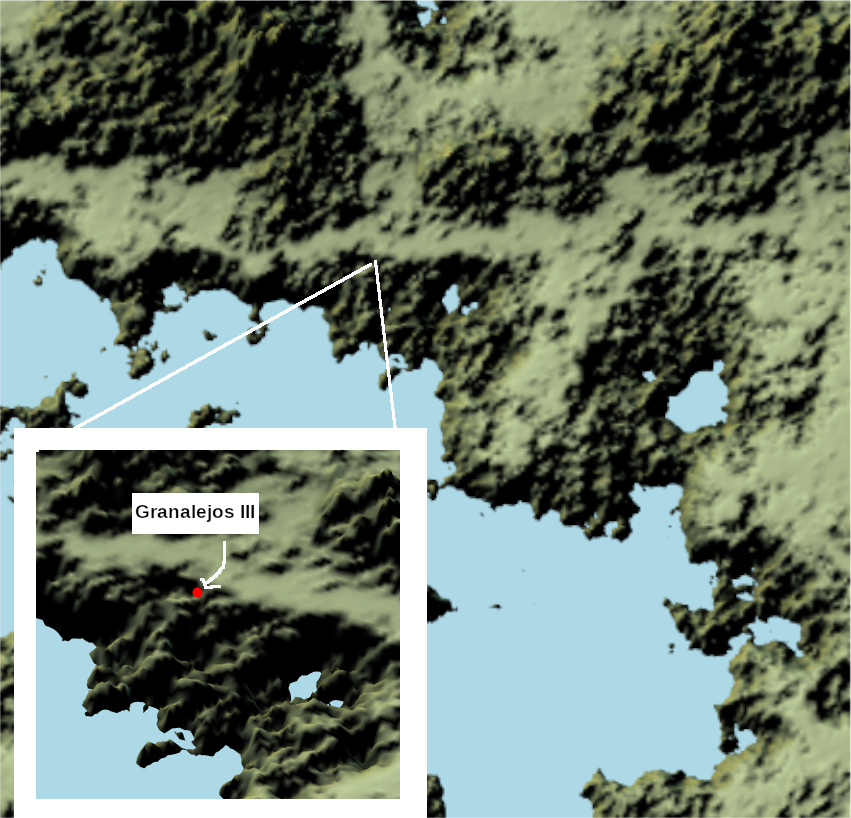
\includegraphics[width=.6\textwidth]{granalejors3}
                }
                \caption{Map of Rabbithole with soome on Granalejos II region's}
            \end{figure}
        \end{block}

        \column{.42\textwidth}
% Create the third block
        \begin{block}{\textbf{Analysis of the Engravings:}}
            

            The engravings on ceramic artifacts were examined using a high-resolution 3D camera. The depictions were classified into different categories based on their subject matter, including battles, weapons, and violent acts. The frequency and distribution of these categories were then analyzed to determine the nature of the interactions between the Poppychewers and Rabbitskinners and did not left any doubt on the conflictual nature of the relationships between Poppychewers and Rabbitskinners. This is totally in line with the very unequal distribution of food resources that Pants~et.~al~(1996) reconstructed.

            \vspace{1cm}
            \begin{figure}
                \label{fig:twomaps}
                \centering
                \makebox[\textwidth][c]{
                    \includegraphics[width=.45\textwidth]{thumbnail_Pot_back}
                    \includegraphics[width=.45\textwidth]{thumbnail_Pot_front_death_marks}
                }
                \caption{New remains from Granalejos II, inside of the pot (left), outside of the pot (right), with detect engravings annotated in red}
            \end{figure}
            \vspace{1cm}



            Our analysis of the engravings gives a unique glimpse into the relationship between the Poppychewers and the Rabbitskinners. This provides compelling evidence of conflict between the ancient populations of Poppychewers and Rabbitskinners. We also examined the depth of the engravings along with style and indicated that one artist used a great deal of force to depict these scenes. Clearly, indicating the degree of animosity the artist felt toward the violence being depicted. Unfortunately, petrographic analysis of the artefact shows that it could have been created anywhere in the valley, and stylistic markers or function indicators were not found, so it is difficult to assess which group this pottery piece came from.

        \end{block}

% Create the fourth block
        \column{.22\textwidth}
    \begin{block}{\textbf{Conclusion}}
        The engravings on the ceramic pottery artefact provide compelling evidence of conflict between the ancient populations of Poppychewers and Rabbitskinners. This discovery challenges previous theories of peaceful coexistence and highlights the importance of analysing archaeological artefacts in their entirety. The engravings offer valuable insights into the dynamics of inter-population relationships and the potential causes of conflict. Future research may shed further light on the specific reasons for this conflict and its impact on the wider region.
        \end{block}

% Create the references block
        \begin{block}{\textbf{References}}
             Pants, F.,\& Stone, H. (1966). Paleo-ecological reconstruction of Rabbitholes environment. Journal of Ecological Research in Ancient Environments, 20(2), 45-56.
        \end{block}
% Create the references block
    \begin{block}{\textbf{Additional note}}
        \small
        This project is part of the Archaoriddle project, it is supported by the MSCA-IF grant no. 101020631 and the BA/Leverhulme grant SRG2223\textbackslash230262. If you want to help us understand what happened between Poppychewers and Rabbitskinners flash the QR-code below. You will have a chance to receive a £650 grant to join us at the EAA in Belfast! 
            \begin{figure}
                \includegraphics[width=.5\textwidth]{qrcode}
            \end{figure}
            {\tiny  All results shown here are derived from simulated dataset, don't reflect any real scenario and should not be take as valid scientific exploration.\\
            }
        \end{block}

    \end{columns}

\end{frame}
\end{document}



